\section{Data}
\label{chap1:sec:data}

This work employs IFS data from the MaNGA survey, part of SDSS-IV \citep{blanton_17_sdss-iv}. MaNGA is the most extensive IFS survey undertaken to date, targeting 10,000 galaxies in the local universe ($0.01 < z < 0.15$), with observations set to complete in early 2020 \citep{bundy15_manga}. MaNGA's instrument is built around the SDSS 2.5-meter telescope at Apache Point Observatory \citep{gunn_sdss_telescope} and the SDSS-BOSS spectrograph \citep{smee_boss_instrument,sdss_boss_dawson_13}, which has a wavelength range of 3600 to 10300 $\mbox{\AA}$ and spectral resolution $R \sim 2000$. The BOSS spectrograph is coupled to close-packed fiber hexabundles (also called integral-field units, or IFUs) with between 19 and 127 fibers subtending 2" apiece on the sky \citep{manga_inst}. The IFUs are secured to the focal plane with a plugplate \citep{sdss_summary}, and are exposed simultaneously. Flux-calibration is accomplished with 12 seven-fiber ``mini-bundles" which observe standard stars simultaneous to science observations \citep{manga_spectrophot}, and sky-subtraction uses 92 single fibers spread across the three-degree focal plane.

MaNGA observations use only dark time, and require three sets of exposures, which are accumulated until a specified threshold signal-to-noise is achieved \citep{manga_progress_yan_16}. Additionally, all constituents of each set of exposures must be taken under similar conditions. A three-point dither pattern is used to increase the spatial sampling such that 99\% of the area within the IFU is exposed to within 1.2\% of the mean exposure time \citep{manga_obs}. This also accomplishes a more uniform sampling of the plane of the sky than non-dithered observations, and gives a closer match to the fiber point-spread function: a typical fiber-convolved point-spread function has FWHM of 2.5" \citep{manga_obs}.

The MaNGA survey primarily targets galaxies from the NASA-Sloan Atlas \texttt{v1\_0\_1} \citep[NSA, ][]{blanton_11_nsa}. The survey's science goals guide the specific target choices made: in particular, two-thirds of targets (the ``Primary+ sample") are covered to 1.5 effective radii ($R_e$), and one-third (the ``Secondary sample") are covered to 2.5 $R_e$. MaNGA targets are selected uniformly in SDSS $i$-band absolute magnitude \citep{fukugita_96_sdss_photo, doi_2010_sdssresponse}, which will result in an approximately-flat distribution in the log of stellar mass \citep{manga_sample_wake_17}. Further, within a prescribed redshift range corresponding to a given absolute magnitude, the MaNGA sample is selected to be volume-limited. Absolute magnitudes have been calculated using K-corrections computed with the \texttt{kcorrect v4\_2} software package \citep{blanton_roweis_07}, assuming a \citet{chabrier03} stellar initial mass function and \citet{BC03} SSPs, and are tabulated in the \texttt{DRPALL} catalog file.

The MaNGA Data Reduction Pipeline \citep[DRP:][]{manga_drp} reduces individual integrations into both row-stacked spectra (RSS), which behave like collections of single-fiber pointings; and rectified data-cubes (CUBE), which are constructed from the RSS with a modified Shepard's algorithm to produce a spatially-uniform grid on the plane of the sky with spaxels measuring 0.5 arcsecond on a side. This work uses CUBE products with logarithmically-uniform wavelength spacing ($d\log \lambda = 10^{-4}$, $d\ln \lambda \approx 2.3 \times 10^{-4}$)\footnote{In this work, the notation $\log$ denotes a base-10 logarithm, and $\ln$ denotes a base-$e$ logarithm.}, also called LOGCUBE products. LOGCUBE products are then analyzed further, using the MaNGA Data Analysis Pipeline \citep[DAP:][]{manga_dap}, which produces resolved measurements (referred to as ``MAPS") of stellar and gas line-of-sight velocity, the stellar continuum, gaseous emission fluxes, and spectral indices.

The \nrungalaxies galaxies analyzed in this study are drawn randomly from \mplvfull (\mplv), an internally-released set of both reduced and analyzed observations numbering \mplvngal galaxies observed between March 2014 and July 2018. \mplv's reduced products number nearly 2100 more than SDSS DR15 \citep{sdss_dr15}, which was released in December 2018. 

This study uses both DRP-LOGCUBE and DAP-MAPS products. The DAP-MAPS products (at this time released only within the SDSS collaboration) are not spatially-binned for the stellar continuum fit \citep[see][]{manga_dap} (i.e., this work uses the ``SPX" products). We apply no sample cuts. The distribution of the median spectral signal-to-noise ratio of all MaNGA spaxels is shown in Figure \ref{fig:spax_snr}: spectral channels flagged at the MaNGA-DRP stage as either having low or no IFU coverage, or with known unreliable measurement, have had their inverse-variance weight set to zero (spaxels with such issues affecting their spectra form the low-SNR tail of the distribution).

\begin{figure}
    \centering
    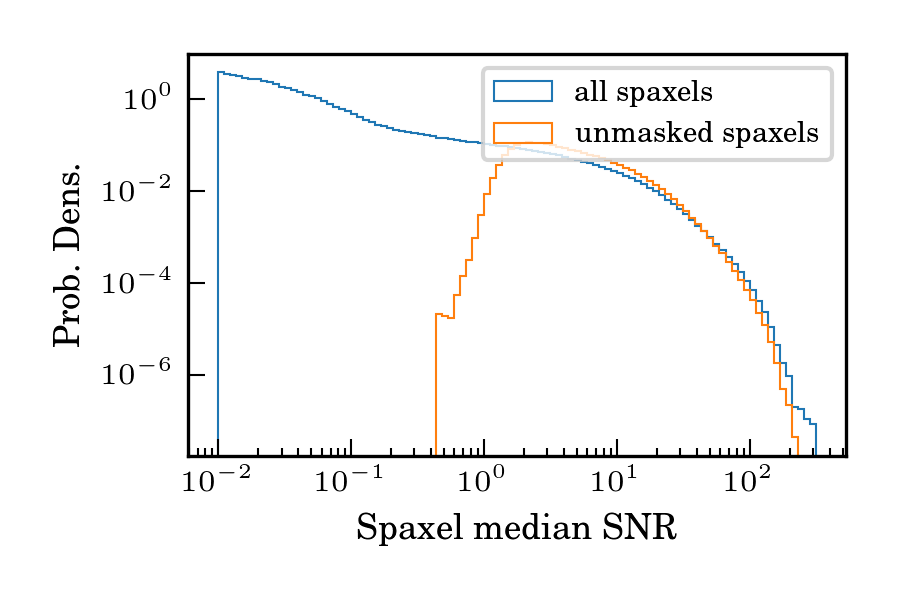
\includegraphics[width=\columnwidth]{spax_snr}
    \caption[Median spaxel signal-to-noise ratios]{\fixspacing The distributions of median spectral signal-to-noise ratio for all MaNGA spaxels (blue) and those spaxels for which none of the MaNGA DRP data-quality flags indicate potential problems with the estimates obtained in this work (orange)---see Section \ref{chap1:subsec:data_quality} for descriptions of data-quality diagnostics, and how channel-specific quality flags inform reliability of mass-to-light ratio estimates.}
    \label{fig:spax_snr}
\end{figure}